\section{List of hardware used} \label{app:hardwareused}

\begin{itemize}
	\item DSLR body (9 units in total): Canon EOS 700D
	\item Lens (one for each camera): Canon EF 50mm f/1.8 II
	\item Power adapter (one for each): Canon ACK-E8
	\item Memory card (one for each): Transcend SDHC class 10 UHS-I 16GB
	\item USB hub (3 units): D-link DUB-H4
	\item Remote board: custom built around ST Nucleo-F401RE, see next section \ref{app:remotetrigger}
	\item Canon RC-6 wireless remote control for testing
	\item Stand (four units): Millenium LST-310, a sturdy three-legged lighting stand with a pole that can be extended several meters high.
	\item Ball head (one for each): Manfrotto 494
	\item Clamp (one for each): Manfrotto 035 Super Clamp, with Manfrotto 036-38 studs
	\item Velcro strap etc. for fastening things
\end{itemize}

\clearpage

\section{Remote trigger} \label{app:remotetrigger}

The remote trigger consists of a Nucleo-F401RE microcontroller platform by ST microelectronics, and supporting hardware for connecting the cameras.
Each camera connects to the trigger via a 2,5mm stereo plug, as the cameras have a standard 2,5mm jack for remote trigger.
To secure the cameras from each other, the remote wires are connected with opto-isolators (TLP621-2).

Much of the physical space is taken by the microcontroller board and the bulky through-hole mounted opto-isolators.
The size of the trigger box could be reduced to approximately half of its size by using surface mount opto-isolators and designing the microcontroller itself on the same circuit board, removing the large pin headers.
This was not a high priority, though, as the whole trigger device is already small compared to the whole system.

\subsection{Schematic} \label{app:fullschematic}

\simplefig{p}{%
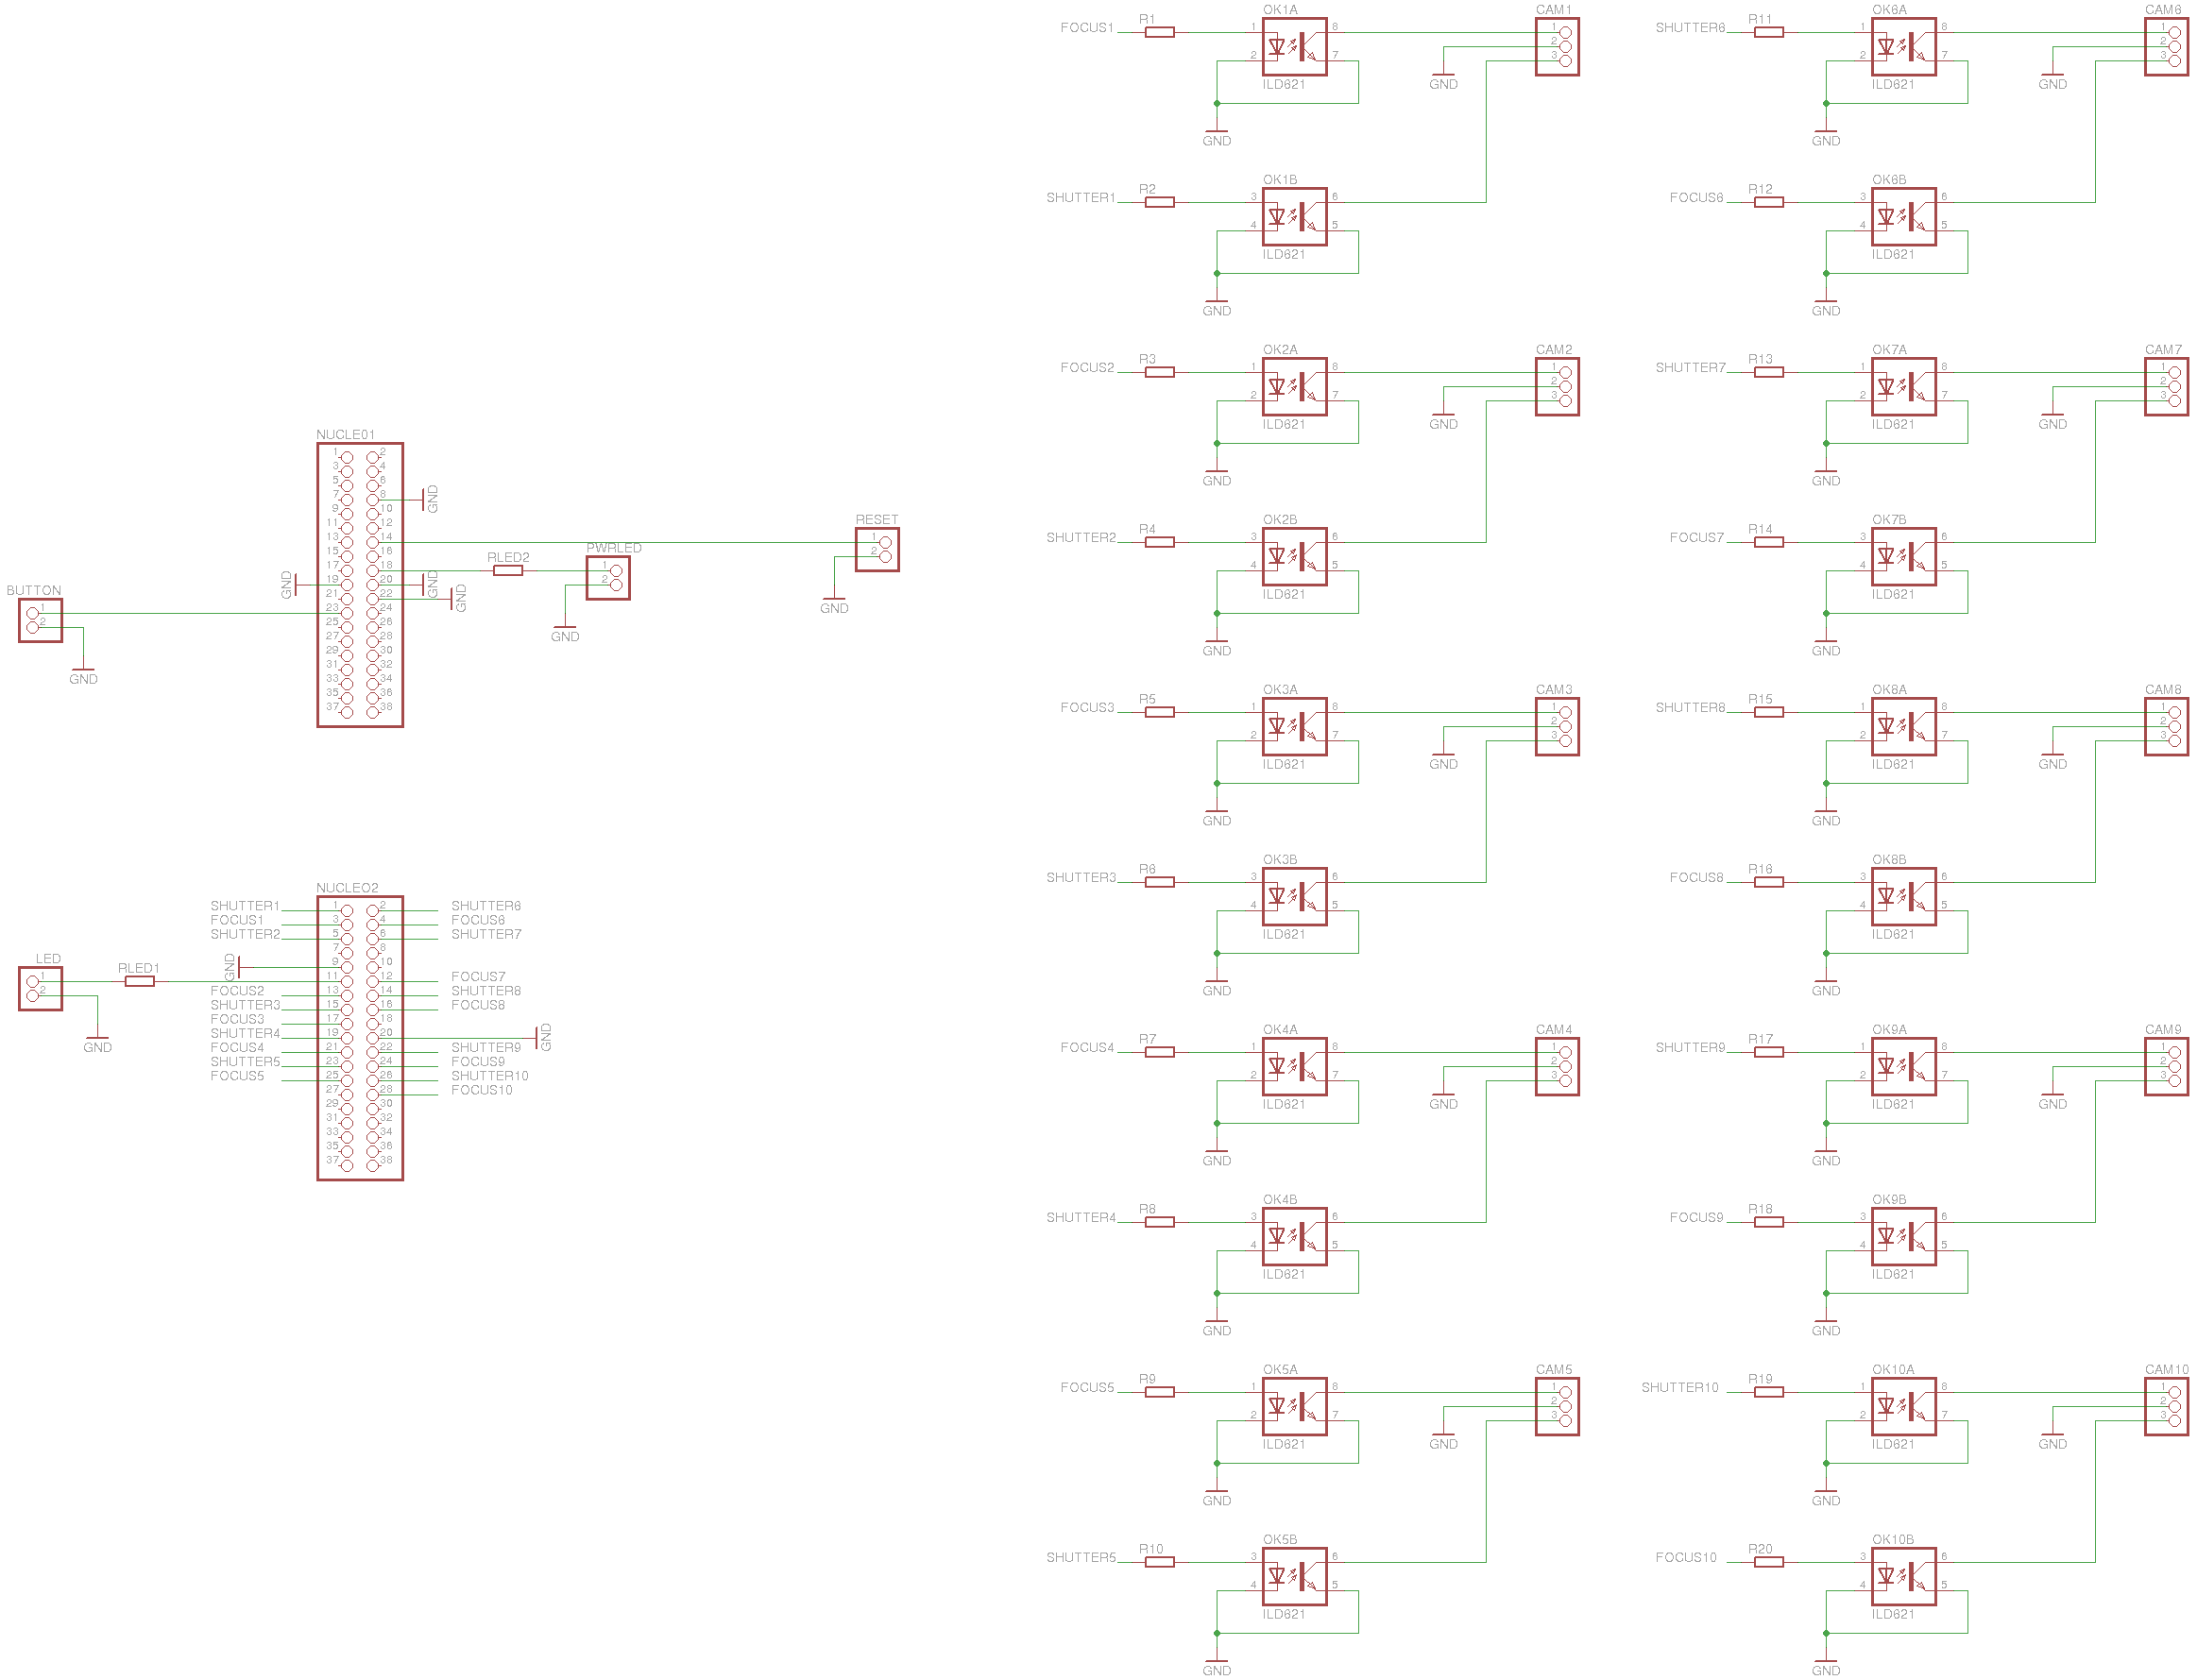
\includegraphics[height=\textwidth, angle=90]{gfx/triggerboard-sch}
}{fig:triggerboard-sch-big}
{Remote trigger schematic}

See figure \ref{fig:triggerboard-sch-big} for a complete schematic.
The two pin headers are those of the Nucleo board, and the order of the opto-isolators and connectors matches with the physical order of the connectors on the PCB.
Additionally, the LEDs and buttons were routed to the side of the board to be accessible when installed in the enclosure.

\subsection{Circuit board layout}

\simplefig{p}{%
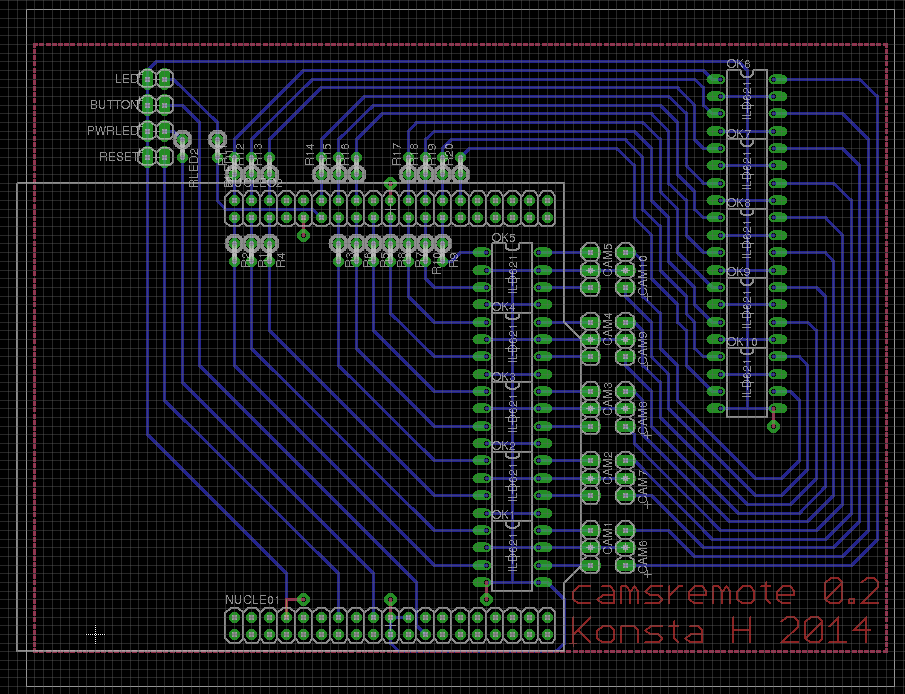
\includegraphics[height=\textwidth, angle=90]{gfx/triggerboard}
}{fig:triggerboard-brd-big}
{Remote trigger circuit board (PCB) layout}

The circuit board dimensions are 5 by 3.9 inches.
All electrical connections can be realized with just one layer;
another layer was used as a ground plane, but the ground signals are routed along with the signals too.
The circuit is also simple enough to implement on e.g. a veroboard with some jumper wires.
Figure \ref{fig:triggerboard-brd-big} shows the board layout without a ground plane.

\subsection{Finished device}

\simplefig{p}{%
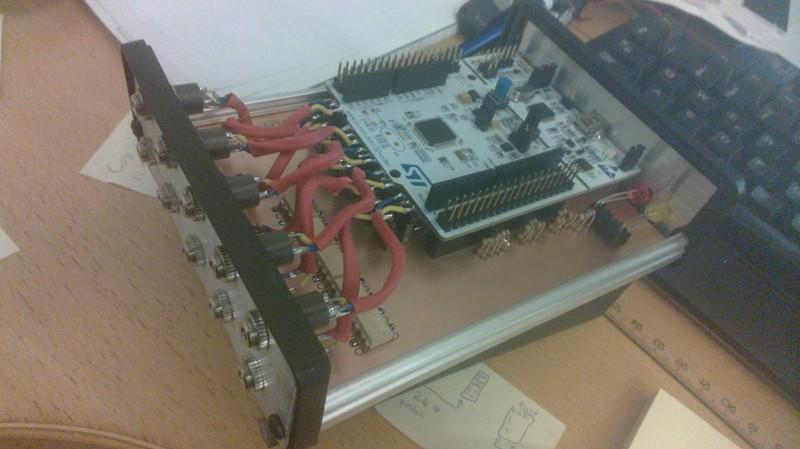
\includegraphics[height=\textwidth, angle=90]{gfx/camsremote}
}{fig:camsremote-full}
{Components installed to the board and fitted in the enclosure (TODO: better pic and closeup of some connectors)}

The PCB was built with a milling machine sold by LPKF Laser \& Electronics AG.
A recycled enclosure was used with custom drilled end caps for the 2,5 mm jacks for the camera connections in one end, and Nucleo board's micro-USB, LEDs and buttons on other end.
\ref{fig:camsremote-full}

\subsection{Parts list}

\begin{itemize}
	\item ST Microelectronics Nucleo-F401RE microcontroller platform
	\item 10 x stereo 2,5 mm jack
	\item 10 x stereo 2,5 mm male-male 3 meter cable
	\item 10 x TLP621-2 opto-isolator; others with similar pinout work too
	\item For an enclosure, two LEDs and pushbuttons should be used
	\item (usb cable, wire, buttons?)
\end{itemize}
